\documentclass[a4paper,14pt]{extreport}
	\usepackage[left=2 cm,right=1.5 cm,
	    top=1.5cm,bottom=2cm,bindingoffset=0cm]{geometry}
	\usepackage{scrextend}
	\usepackage[T1,T2A]{fontenc}
	\usepackage[utf8]{inputenc}
	\usepackage[russian,ukrainian,english]{babel}
	\usepackage{tabularx}
	\linespread{1.5}
	\usepackage{amssymb}
	\usepackage{color}
	\usepackage{amsmath}
	\usepackage{mathrsfs}
	\usepackage{listings}
	\usepackage{graphicx}
	\graphicspath{ {./images/} }
	\usepackage{lipsum}
	\usepackage{xcolor}
	\usepackage{hyperref}
	\usepackage{tcolorbox}
	\usepackage{tikz}
	\usepackage[framemethod=TikZ]{mdframed}
	\usepackage{wrapfig,boxedminipage,lipsum}
	\mdfdefinestyle{MyFrame}{%
	linecolor=blue,outerlinewidth=2pt,roundcorner=20pt,innertopmargin=\baselineskip,innerbottommargin=\baselineskip,innerrightmargin=20pt,innerleftmargin=20pt,backgroundcolor=gray!50!white}
	 \usepackage{csvsimple}
	 \usepackage{supertabular}
	\usepackage{pdflscape}
	\usepackage{fancyvrb}
	%\usepackage{comment}
	\usepackage{array,tabularx}
	\usepackage{colortbl}

	\usepackage{varwidth}
	\tcbuselibrary{skins}
	\usepackage{fancybox}


	\usepackage{tikz}
	\usepackage[framemethod=TikZ]{mdframed}
	\usepackage{xcolor}
	\usetikzlibrary{calc}
	\makeatletter
	\newlength{\mylength}
	\xdef\CircleFactor{1.1}
	\setlength\mylength{\dimexpr\f@size pt}
	\newsavebox{\mybox}
	\newcommand*\circled[2][draw=blue]{\savebox\mybox{\vbox{\vphantom{WL1/}#1}}\setlength\mylength{\dimexpr\CircleFactor\dimexpr\ht\mybox+\dp\mybox\relax\relax}\tikzset{mystyle/.style={circle,#1,minimum height={\mylength}}}
	\tikz[baseline=(char.base)]
	\node[mystyle] (char) {#2};}
	\makeatother

	\definecolor{ggreen}{rgb}{0.4,1,0}
	\definecolor{rred}{rgb}{1,0.1,0.1}
	\definecolor{amber}{rgb}{1.0, 0.75, 0.0}
	\definecolor{babyblue}{rgb}{0.54, 0.81, 0.94}
	\definecolor{asparagus}{rgb}{0.53, 0.66, 0.42}
	\definecolor{chartreuse}{rgb}{0.5, 1.0, 0.0}
	\definecolor{darkorchid}{rgb}{0.6, 0.2, 0.8}

	\usepackage{float}
	\usepackage{wrapfig}
	\usepackage{framed}
	%for nice Code{
	\lstdefinestyle{customc}{
	  belowcaptionskip=1\baselineskip,
	  breaklines=true,
	  frame=L,
	  xleftmargin=\parindent,
	  language=C,
	  showstringspaces=false,
	  basicstyle=\small\ttfamily,
	  keywordstyle=\bfseries\color{green!40!black},
	  commentstyle=\itshape\color{purple!40!black},
	  identifierstyle=\color{blue},
	  stringstyle=\color{orange},
	}
	\lstset{escapechar=@,style=customc}
%}


\begin{document}
\pagecolor{white}

%----------------------------------------1
\newtcbox{\xmybox}[1][red]{on line, arc=7pt,colback=#1!10!white,colframe=#1!50!black, before upper={\rule[3pt] {0pt}{10pt}},boxrule=1pt,boxsep=0pt,left=6pt,right=6pt,top=2pt,bottom=2pt}

\begin{center}\xmybox[green]{Mnatsakanov Anton} \xmybox[amber]{DP-82} \xmybox[blue]{Variant №5}
\vspace{1cm}

\end{center}


\begin{center}Опішить механізм стримірної теорії пробою. Коли спостерігається оптичний пробій?\end{center}

In general, the theory of streamer breakdown was developed by G. Reuter, L. Leb and J. Meek and
as we know the streamer is a flux of positive volumetric charge that arises and moves in gases under the action of an electric field. This flux violates the homogeneity of the electric field, attracts electrons and spreads due to the processes of photoionization.
The emergence and propagation of streamer in the discharge gap \\
 is explained by Fig. \ Ref {r1}, which is like a series of four "snapshots" of the same discharge gap, taken at small time intervals.
\begin{figure}[h]
	\center{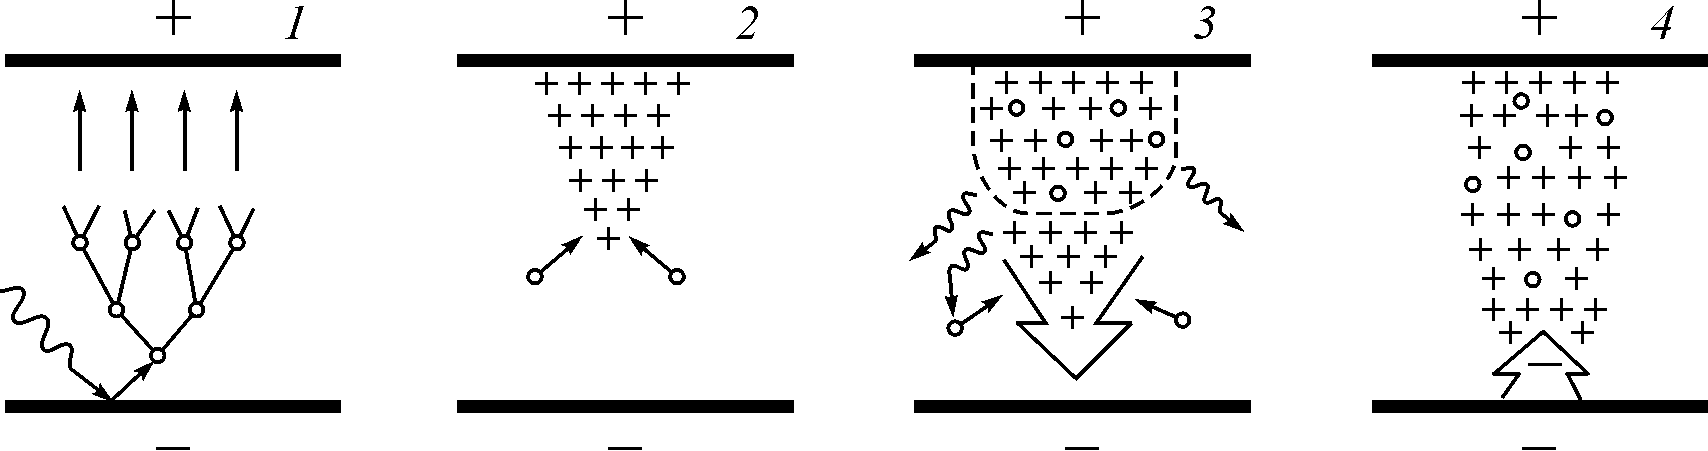
\includegraphics[width=0.9\linewidth]{1.png}}
	\caption{ To explain the mechanism of streamer breakdown: o - electron, + - positive ion, $ \rightsquigarrow$ - photon}
	\label{r1}
\end{figure}\par

1. Due to an external ionizer (for example, in the case of photoemission with a cathode) an electron appeared in the cathode-anode gap, which generates the initial electron Avalanche. The avalanche propagates toward the anode at a velocity of about 10$^6$ m/s. \\

2. Fast electrons moving under the influence of strong electric field at the anode, left behind a cloud of relatively motionless positive ions (whose mass compared with electron dynamics is very large). This cloud, as follows an avalanche, has an overview as if a tip and is a needle-like continuation of the anode. Then not far from the voltage of the electric field is increased, and therefore the electricity providing the discharge gap with one reason or another, with great acceleration are attracted to the tip. \\

3. electrons fly into the region of positive-volumetric charge near the tip, recombine with acting ions, generating photoviprominution, especially intensive near the streamer head. This radiation leads to secondary photoionization, due to which new electron avalanches are born. Thus, the streamer moves from the anode to the cathode, and photoelectrons, which bind in the region of positive charge, create together with positive ions an electrically conductive plasma. The streamer propagation velocity is estimated to be large 10$^6$ m/s. \\

4. The streamer that grows from the anode reaches the cathode, causing the plasma channel to close the discharge gap. As a result, a powerful wave of electric current is amplified from the code, which appears in the discharge gap as a spark (in the case of low power voltage sources), or an electric arc is ignited (provided the voltage source power is large enough to support vaporization as well as a powerful long discharge ). The velocity of the spark is about 10$^7$ m/s. \\

The breakdown voltage value, which characterizes a streamer breakdown, \\ is determined under conditions of self-propagation of the streamer and resistance to ionization of atoms or gas molecule. When the field is small, the streamer cannot join, so that only clouds of positive ions are created (due to random electron avalanches), which are quickly dealt with by diffusion in the gas. The most important condition for the use and diffusion of the streamer is to support the photoionization process in the gas volume. If the electric voltage becomes high for so many processes, it will have a corresponding electrical breakdown. \\

The time interval characterizing the development of such a single lavin probiotic is also determined by the photoionization processes (it has already been determined above that this time is two orders of magnitude shorter than in the case of a taunsendivsic breakdown). Indeed, the time interval, the development of the one-lavin light electron breakdown (about 10$^{-6}$ s) can in no way respond to the movement in the discharge gap of über and important positive ions. On the other hand, the photo propagation speed (speed of light) corresponds to a significant measure of the time interval (in 10$^{-10}$ s), which also does not threaten the experiment. In fact, the streamer breakdown time creates ionization and recombination processes, it is the lifetime of an excited molecule to emit light quanta. It is this time (about 10$^{-8}$ s) that determines the rate of propagation of the single-valve breakdown. \\

Gas breakdown is part of the physics of the gas discharge. Only the basic laws of gas breakdown in homogeneous electric fields have been considered above. Peculiarities of gas breakdown in inhomogeneous electric fields will be considered in high voltage engineering. High-frequency breakdown of gases also has its own characteristics and needs microwave technology. In the case of microwave breakdown of electricity, attached to a strong and rapidly changing (often 10$^{8}$ ... 10$^{10}$ Hz) electric field is not subject to the electrodes, and the amount in the region, generates plasma and world .
It is believed that the phenomenon of ball lightning is also displayed with ultrahigh frequency processes in the discharge plasma. Vijay, to the gas breakdown recovery and the phenomenon of atmospheric electricity. Therefore, lightning is the longest electrical connection, which also begins with a streamer. It spreads out in rapid-onset one after another gait has a length of several meters. The streamer's motion in this case is discontinuous, for its average velocity is less than in a uniform field, and is about 10$^{5}$ m/s. The streamer offers an electrically conductive channel, after which the velocity to 10$^{8}$ m / s is then amplified by a powerful spark (current strength sets hundreds of amperes). The diameter of the lightning discharge channel to account for heat instantly expands to 0.1 ... 0.2 m, and the difference in pressure increase in this channel creates a shock wave (thunder). \\

Thus, the streamer theory satisfactorily explains the main regularities of the single-valve breakdown in gases. It should also be noted that the main ideas of the streamer breakdown mechanism are also used to explain the electronic breakdown of liquid and solid dielectrics. \\

Optical breakdown of transparent dielectrics is facilitated by the presence of defects and self-focusing of the laser beam in the dielectric. An ionization wave is generated near the defects in the structure or local heating occurs, destroying the dielectric. Self-focusing of light is a phenomenon of light wave field concentration in a nonlinear medium whose refractive index depends on the field intensity. Due to the nonlinear change in the electronic polarization of the substance, the refractive index of the medium increases with the growth of the field. The structure of the laser pulse is naturally such that the maximum light intensity is in the central region of the beam. \\

Two mechanisms of optical breakdown are possible. The first of them does not differ in its nature from the breakdown of gases in fields of not very high frequencies (this includes the microwave range). The first (bare) electrons appearing for one reason or another, absorbing photons, gain energy. Having accumulated energy sufficient for ionization, the electrons ionize atoms - an avalanche develops. In strong fields, this process takes place fairly quickly and a breakdown occurs in the gas. \\

The second mechanism of optical breakdown is purely quantum in nature. Electrons can bounce off atoms as a result of the many-quantum
photoeffect, i.e. in case of simultaneous absorption of several photons at once. One-quantum photoeffect in the case of visible range frequencies is impossible because the ionization potentials of atoms are several times greater than the energy of the quantum. For example, the photon energy of a ruby laser is 1.8 eV, while the ionization potential of argon is 16 eV, i.e. 9 photons are required for electron detachment. The rate of multiphoton processes increases dramatically with increasing photon flux density. However, at pressures on the order of atmospheric pressure, avalanche ionization is more likely, and multiphoton processes only cause the appearance of initial electrons.




\end{document}
